\documentclass[aspectratio=169,10pt]{beamer}
\input{../../template/pdp-beamer.sty}
\pdpfooter{Metode Numerik PDP Orde Dua}{}

\title{Metode Beda Hingga untuk PDP Parabolik dan Eliptik}
\subtitle{Stabilitas, Konvergensi, dan Verifikasi terhadap Solusi Analitik}
\author{Tim Pengajar Persamaan Diferensial Parsial}
\institute{Program Studi Matematika - Institut Teknologi Sumatera}
\date{Pertemuan 12}

\begin{document}

% 1 -----------------------------------------------------------------
\begin{frame}[plain]
  \begin{tikzpicture}[remember picture,overlay]
    \fill[pdpNavy] (current page.south west) rectangle ([xshift=0.33\paperwidth]current page.north west);
    \fill[pdpTeal] ([xshift=0.33\paperwidth]current page.south west) rectangle ([xshift=0.337\paperwidth]current page.north west);
  \end{tikzpicture}
  \vspace{0.62cm}
  \begin{columns}[T]
    \column{0.30\textwidth}
      \color{white}
      {\bfseries MA 25-31018}\par\vspace{0.25cm}
      {\Large\bfseries PERSAMAAN\\ DIFERENSIAL\\ PARSIAL}\par\vspace{0.95cm}
      {\color{pdpMint}\large\bfseries Pertemuan 12}
    \column{0.64\textwidth}
      {\LARGE\bfseries Metode Beda Hingga untuk PDP Parabolik dan Eliptik}\par
      \pdporangeline
      {\large Stabilitas, Konvergensi, dan Verifikasi terhadap Solusi Analitik}\par\vspace{0.48cm}
      {\bfseries Koordinator:} Dear Michiko Mutiara Noor, M.Si.\par
      {\bfseries Tim pengajar:} Dr. Dewi Suhika, M.Sc. dan Rifky Fauzi\par\vspace{0.62cm}
      Program Studi Matematika\par
      Institut Teknologi Sumatera
  \end{columns}
\end{frame}

% 2 -----------------------------------------------------------------
\begin{frame}{Keterkaitan dengan Materi Analitik Sebelumnya}
\small
\begin{columns}[T,onlytextwidth]
\column{0.24\textwidth}
\begin{block}{Deret Fourier I}
Basis periodik
\[
1,\cos nx,\sin nx
\]
dan koefisien pada $(-\pi,\pi)$.
\end{block}
\column{0.24\textwidth}
\begin{block}{Deret Fourier II}
Skala domain menjadi
\[
(-L,L)
\]
dengan basis $\cos(n\pi x/L)$ dan $\sin(n\pi x/L)$.
\end{block}
\column{0.24\textwidth}
\begin{block}{Deret Fourier III}
Perluasan genap/ganjil menghasilkan deret kosinus/sinus pada $(0,L)$.
\end{block}
\column{0.24\textwidth}
\begin{block}{Persamaan Panas}
Separasi variabel menghasilkan mode eigen yang sama, dengan amplitudo yang meluruh terhadap waktu.
\end{block}
\end{columns}
\vspace{0.12cm}
\begin{beamercolorbox}[sep=.12cm,wd=\textwidth]{normal text}
\centering
Materi numerik hari ini \textbf{tidak mengganti analitik}. Solusi analitik menjadi acuan untuk menilai apakah skema diskret benar dan cukup akurat.
\end{beamercolorbox}
\pdpsource{Prasyarat materi: Deret Fourier (I)--(III) dan Persamaan Panas--Separasi Variabel, D. Michiko M. Noor, 2026.}
\end{frame}

% 3 -----------------------------------------------------------------
\begin{frame}{Persamaan Panas: Masalah Nilai Awal-Batas yang Menjadi Acuan}
\small
Mengikuti notasi materi analitik, ambil $k>0$ sebagai difusivitas:
\[
\boxed{u_t-k u_{xx}=0},\qquad 0<x<L,\ t>0,
\]
\[
 u(0,t)=u(L,t)=0,\qquad u(x,0)=\phi(x).
\]
\begin{columns}[T,onlytextwidth]
\column{0.48\textwidth}
\begin{block}{Mengapa hanya satu kondisi awal?}
Persamaan panas berorde satu terhadap waktu. Setelah $u(x,0)=\phi(x)$ diketahui, nilai awal $u_t(x,0)$ tidak bebas; dari PDP,
\[
 u_t(x,0)=k\,\phi''(x)
\]
bila $\phi$ cukup halus.
\end{block}
\column{0.48\textwidth}
\begin{block}{Bandingkan dengan persamaan gelombang}
Persamaan gelombang berorde dua terhadap waktu, sehingga memerlukan dua data awal independen:
\[
 u(x,0),\qquad u_t(x,0).
\]
Perbedaan ini berasal langsung dari orde turunan waktu.
\end{block}
\end{columns}
\end{frame}

% 4 -----------------------------------------------------------------
\begin{frame}{Separasi Variabel dan Basis Eigen untuk Persamaan Panas}
\footnotesize
Ambil bentuk terpisah
\[
 u(x,t)=X(x)T(t).
\]
Substitusi ke $u_t-k u_{xx}=0$ memberi
\[
 X T'-kX''T=0
 \quad\Longrightarrow\quad
 \frac{T'}{kT}=\frac{X''}{X}=-\lambda.
\]
Tanda $-\lambda$ dipilih karena syarat batas $X(0)=X(L)=0$ memiliki solusi nontrivial untuk $\lambda>0$:
\[
 X''+\lambda X=0,\qquad X(0)=X(L)=0.
\]
Diperoleh
\[
 \lambda_n=\left(\frac{n\pi}{L}\right)^2,
 \qquad X_n(x)=\sin\left(\frac{n\pi x}{L}\right),
\]
\[
 T_n(t)=\exp\!\left[-k\left(\frac{n\pi}{L}\right)^2t\right].
\]
Karena PDP linear, superposisi mode juga solusi:
\[
\boxed{u(x,t)=\sum_{n=1}^{\infty} b_n
 e^{-k(n\pi/L)^2t}\sin\left(\frac{n\pi x}{L}\right)}.
\]
\end{frame}

% 5 -----------------------------------------------------------------
\begin{frame}{Koefisien Fourier Menentukan Kondisi Awal}
\small
Pada $t=0$,
\[
 \phi(x)=u(x,0)=\sum_{n=1}^{\infty}b_n\sin\left(\frac{n\pi x}{L}\right).
\]
Ini tepat deret sinus yang muncul dari \textbf{perluasan ganjil} fungsi pada $(0,L)$. Dengan ortogonalitas sinus,
\[
\boxed{b_n=\frac{2}{L}\int_0^L \phi(x)
\sin\left(\frac{n\pi x}{L}\right)\,dx}.
\]
\begin{columns}[T,onlytextwidth]
\column{0.48\textwidth}
\begin{block}{Benchmark satu mode}
Pilih
\[
\phi(x)=\sin\left(\frac{\pi x}{L}\right).
\]
Maka $b_1=1$ dan $b_n=0$ untuk $n\ge2$.
\end{block}
\column{0.48\textwidth}
\begin{block}{Solusi eksak}
\[
\boxed{u(x,t)=e^{-k(\pi/L)^2t}
\sin\left(\frac{\pi x}{L}\right)}.
\]
Inilah benchmark utama untuk memeriksa skema numerik.
\end{block}
\end{columns}
\end{frame}

% 6 -----------------------------------------------------------------
\begin{frame}{Diskretisasi Ruang dan Waktu}
\small
Bagi domain menjadi grid seragam:
\[
 x_i=i h,\qquad h=\frac{L}{N},\qquad
 t^n=n\,\Delta t,
\]
dan tulis
\[
 U_i^n\approx u(x_i,t^n).
\]
Dari ekspansi Taylor terhadap waktu,
\[
 u(x_i,t^{n+1})=u(x_i,t^n)+\Delta t\,u_t(x_i,t^n)+O(\Delta t^2),
\]
sehingga
\[
 u_t(x_i,t^n)=\frac{U_i^{n+1}-U_i^n}{\Delta t}+O(\Delta t).
\]
Dari Taylor terhadap ruang di $x_i$,
\[
 u(x_i\!\pm\! h,t^n)=u_i^n\pm h u_x+\frac{h^2}{2}u_{xx}\pm\frac{h^3}{6}u_{xxx}+O(h^4),
\]
sehingga setelah dijumlahkan,
\[
 u_{xx}(x_i,t^n)=\frac{U_{i+1}^n-2U_i^n+U_{i-1}^n}{h^2}+O(h^2).
\]
\end{frame}

% 7 -----------------------------------------------------------------
\begin{frame}{Skema FTCS dan Konsistensi}
\small
Substitusikan dua aproksimasi sebelumnya ke $u_t=k u_{xx}$:
\[
 \frac{U_i^{n+1}-U_i^n}{\Delta t}
 =k\frac{U_{i+1}^n-2U_i^n+U_{i-1}^n}{h^2}.
\]
Definisikan bilangan tak berdimensi
\[
\boxed{r=\frac{k\Delta t}{h^2}}.
\]
Maka skema \textbf{Forward Time--Centered Space (FTCS)} adalah
\[
\boxed{U_i^{n+1}=U_i^n+r\left(U_{i+1}^n-2U_i^n+U_{i-1}^n\right)}.
\]
\begin{block}{Konsistensi}
Galat pemotongan berasal dari suku Taylor yang dibuang:
\[
\tau_i^n=O(\!\Delta t)+O(h^2).
\]
Karena $\tau_i^n\to0$ ketika $\Delta t,h\to0$, FTCS konsisten terhadap persamaan panas.
\end{block}
\end{frame}

% 8 -----------------------------------------------------------------
\begin{frame}{Stabilitas FTCS melalui Mode Diskret}
\footnotesize
Materi Fourier menunjukkan bahwa fungsi dapat diuraikan menjadi mode sinus. Untuk grid Dirichlet, ambil satu mode diskret
\[
 U_i^n=A_n\sin\left(\frac{m\pi i}{N}\right),\qquad m=1,2,\dots,N-1.
\]
Substitusi ke FTCS menghasilkan
\[
 A_{n+1}=G_m A_n,
\]
dengan \textbf{faktor amplifikasi}
\[
\boxed{G_m=1-4r\sin^2\left(\frac{m\pi}{2N}\right)}.
\]
$G_m$ mengukur perubahan amplitudo satu mode dalam satu langkah waktu. Agar gangguan numerik tidak membesar terus-menerus, diperlukan
\[
 |G_m|\le1\qquad\text{untuk semua }m.
\]
Nilai terburuk terjadi pada mode grid berfrekuensi tinggi, sehingga
\[
 -1\le 1-4r\le1
 \quad\Longrightarrow\quad
\boxed{0\le r\le\frac12}.
\]
Jadi FTCS stabil hanya jika $k\Delta t/h^2\le1/2$ untuk model 1D ini.
\end{frame}

% 9 -----------------------------------------------------------------
\begin{frame}{Ketidakstabilan ketika Syarat FTCS Dilanggar}
\begin{columns}[T,onlytextwidth]
\column{0.56\textwidth}
\centering
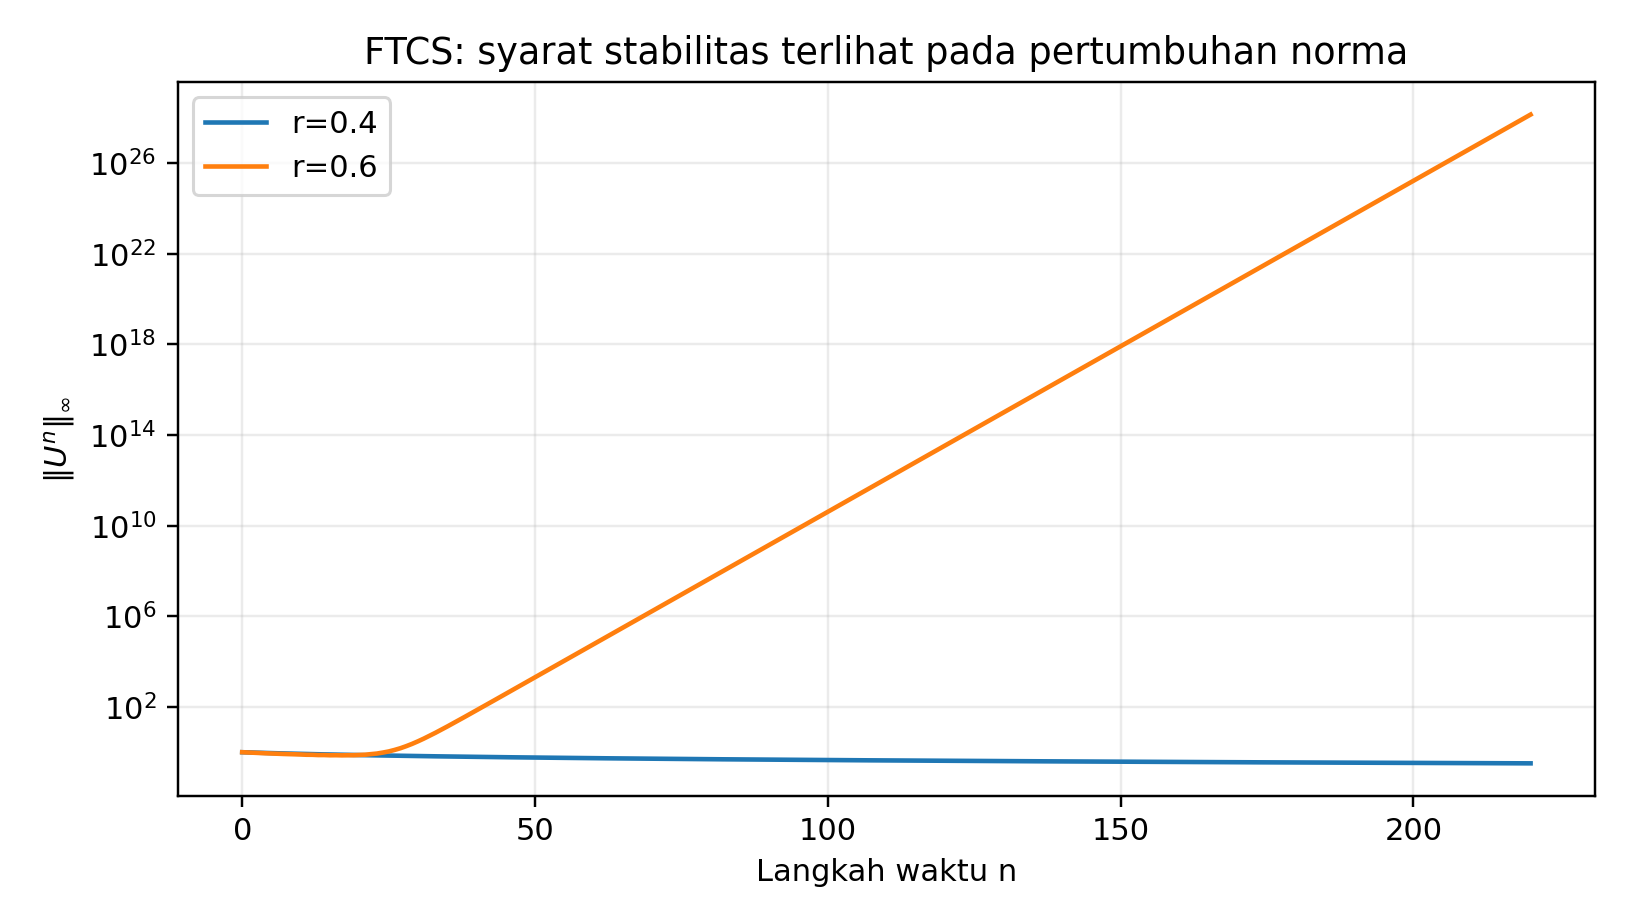
\includegraphics[width=\linewidth,height=4.7cm,keepaspectratio]{figures/heat_ftcs_unstable.png}
\column{0.41\textwidth}
\small
\begin{block}{Apa yang terjadi?}
Untuk $r>1/2$, terdapat mode dengan
\[
|G_m|>1.
\]
Kesalahan pembulatan, diskretisasi, atau gangguan kecil pada mode tersebut diperbesar setiap langkah waktu.
\end{block}
\begin{block}{Makna jangka panjang}
Walaupun beberapa langkah awal dapat tampak masuk akal, amplitudo numerik akhirnya tumbuh dan tidak lagi merepresentasikan solusi difusi yang seharusnya meluruh.
\end{block}
\end{columns}
\end{frame}

% 10 ----------------------------------------------------------------
\begin{frame}{Backward Euler: Skema Implisit}
\footnotesize
Gunakan beda mundur untuk turunan waktu pada $t^{n+1}$:
\[
 u_t(x_i,t^{n+1})\approx\frac{U_i^{n+1}-U_i^n}{\Delta t}.
\]
Evaluasi operator ruang juga pada $t^{n+1}$:
\[
 \frac{U_i^{n+1}-U_i^n}{\Delta t}
 =k\frac{U_{i+1}^{n+1}-2U_i^{n+1}+U_{i-1}^{n+1}}{h^2}.
\]
Dengan $r=k\Delta t/h^2$,
\[
\boxed{-rU_{i-1}^{n+1}+(1+2r)U_i^{n+1}-rU_{i+1}^{n+1}=U_i^n}.
\]
Semua nilai pada waktu baru saling terkopel; karena itu setiap langkah memerlukan penyelesaian sistem linear tridiagonal.
\begin{block}{Stabilitas mode}
Untuk mode sinus yang sama,
\[
\boxed{G_m=\frac{1}{1+4r\sin^2(m\pi/(2N))}}.
\]
Untuk setiap $r>0$, berlaku $0<G_m\le1$. Maka Backward Euler stabil tanpa batasan $r$ untuk persamaan panas linear ini.
\end{block}
\end{frame}

% 11 ----------------------------------------------------------------
\begin{frame}{Crank--Nicolson: Rata-rata Waktu Orde Dua}
\footnotesize
Crank--Nicolson memakai rata-rata operator difusi pada $t^n$ dan $t^{n+1}$:
\[
\frac{U_i^{n+1}-U_i^n}{\Delta t}
=\frac{k}{2h^2}\Big[
(U_{i+1}^{n+1}-2U_i^{n+1}+U_{i-1}^{n+1})
+(U_{i+1}^{n}-2U_i^{n}+U_{i-1}^{n})\Big].
\]
Dengan $r=k\Delta t/h^2$, bentuk aljabarnya
\[
-rU_{i-1}^{n+1}+2(1+r)U_i^{n+1}-rU_{i+1}^{n+1}
=
 rU_{i-1}^{n}+2(1-r)U_i^{n}+rU_{i+1}^{n}.
\]
Skema ini memiliki galat pemotongan
\[
 O(\Delta t^2+h^2).
\]
Untuk mode sinus,
\[
\boxed{G_m=\frac{1-2r\sin^2(m\pi/(2N))}{1+2r\sin^2(m\pi/(2N))}},
\qquad |G_m|\le1\ \text{untuk semua }r>0.
\]
Namun untuk $r$ sangat besar, mode frekuensi tinggi dapat memiliki $G_m\approx-1$: amplitudo tidak tumbuh, tetapi tanda berganti sehingga dapat muncul osilasi transien.
\end{frame}

% 12 ----------------------------------------------------------------
\begin{frame}{Stabilitas Tidak Identik dengan Akurasi}
\begin{columns}[T,onlytextwidth]
\column{0.52\textwidth}
\centering
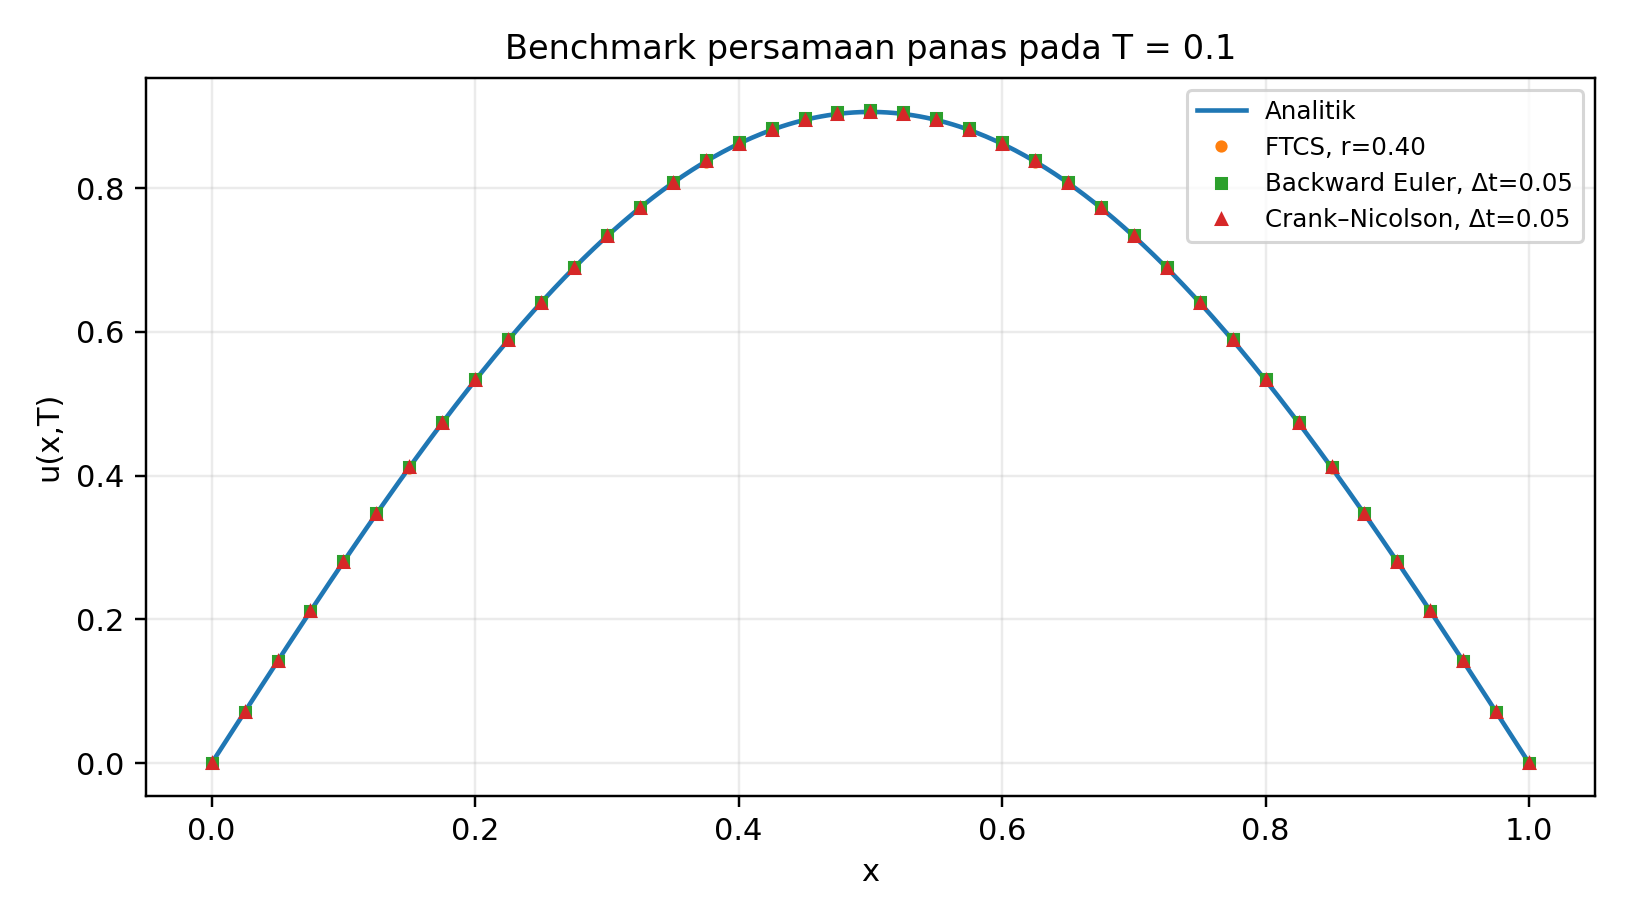
\includegraphics[width=\linewidth,height=3.8cm,keepaspectratio]{figures/heat_benchmark.png}
\column{0.45\textwidth}
\footnotesize
\begin{block}{Tiga pertanyaan berbeda}
\textbf{Konsisten:} apakah persamaan diskret mendekati PDP ketika grid diperhalus?

\vspace{0.08cm}
\textbf{Stabil:} apakah gangguan kecil tetap terkendali sepanjang komputasi?

\vspace{0.08cm}
\textbf{Akurat:} pada grid yang dipakai sekarang, seberapa dekat $U$ dengan solusi PDP?
\end{block}
\begin{block}{Konsekuensi}
Backward Euler dapat stabil untuk $\Delta t$ besar, tetapi error waktunya masih dapat besar. Crank--Nicolson berorde waktu lebih tinggi, tetapi data tidak mulus dapat menghasilkan osilasi transien.
\end{block}
\end{columns}
\end{frame}

% 13 ----------------------------------------------------------------
\begin{frame}{Konsistensi, Stabilitas, dan Konvergensi}
\small
\begin{columns}[T,onlytextwidth]
\column{0.31\textwidth}
\begin{block}{Konsistensi}
Jika solusi eksak dimasukkan ke skema, residual diskret atau galat pemotongan memenuhi
\[
\tau_{h,\Delta t}\to0
\]
ketika $h,\Delta t\to0$.
\end{block}
\column{0.31\textwidth}
\begin{block}{Stabilitas}
Gangguan kecil pada data awal, boundary, atau pembulatan tidak diperbesar tanpa kendali oleh skema diskret.
\end{block}
\column{0.31\textwidth}
\begin{block}{Konvergensi}
Pada waktu tetap $t^n$,
\[
\max_i|U_i^n-u(x_i,t^n)|\to0
\]
ketika grid diperhalus.
\end{block}
\end{columns}
\vspace{0.13cm}
\begin{beamercolorbox}[sep=.12cm,wd=\textwidth]{normal text}
\small
\textbf{Teorema ekuivalensi Lax--Richtmyer.} Untuk masalah nilai awal linear yang \emph{well-posed} dan skema beda hingga yang konsisten, stabilitas ekuivalen dengan konvergensi. \emph{Well-posed} berarti solusi ada, unik, dan bergantung kontinu pada data.
\end{beamercolorbox}
\pdpsource{Lax, P.D. \& Richtmyer, R.D. (1956), Communications on Pure and Applied Mathematics 9, 267--293.}
\end{frame}

% 14 ----------------------------------------------------------------
\begin{frame}{Verifikasi Numerik dan Validasi Model}
\small
\begin{columns}[T,onlytextwidth]
\column{0.48\textwidth}
\begin{block}{Verifikasi}
Pertanyaan: \textbf{apakah persamaan matematika diselesaikan dengan benar?}

\vspace{0.08cm}
Gunakan:
\begin{itemize}
  \item solusi analitik;
  \item manufactured solution;
  \item grid/time-step refinement;
  \item pemeriksaan orde galat.
\end{itemize}
\end{block}
\column{0.48\textwidth}
\begin{block}{Validasi}
Pertanyaan: \textbf{apakah model matematika cukup merepresentasikan fenomena yang dituju?}

\vspace{0.08cm}
Gunakan perbandingan dengan:
\begin{itemize}
  \item data eksperimen;
  \item observasi lapangan;
  \item data pasar;
  \item benchmark fisik yang relevan.
\end{itemize}
\end{block}
\end{columns}
\vspace{0.12cm}
\centering
\textbf{Solusi numerik dapat terverifikasi tetapi modelnya belum tentu tervalidasi.}
\pdpsource{Roache (2002), Journal of Fluids Engineering 124(1), 4--10; terminology aligned with ASME V\&V.}
\end{frame}

% 15 ----------------------------------------------------------------
\begin{frame}{Black--Scholes sebagai PDP Parabolik}
\footnotesize
Untuk opsi call Eropa, $V(S,t)$ menyatakan nilai kontrak ketika harga aset adalah $S$ pada waktu $t$. Model klasik memenuhi
\[
\boxed{V_t+\frac12\sigma^2S^2V_{SS}+rSV_S-rV=0},
\]
dengan kondisi terminal
\[
V(S,T)=\max(S-K,0).
\]
\begin{columns}[T,onlytextwidth]
\column{0.47\textwidth}
\begin{block}{Makna simbol}
$K$: strike price; $T$: maturity; $r$: suku bunga bebas risiko; $\sigma$: volatilitas; $V_{SS}$: kelengkungan nilai opsi terhadap harga aset.
\end{block}
\column{0.49\textwidth}
\begin{block}{Struktur PDP}
\begin{itemize}
  \item $V_t$: perubahan terhadap waktu;
  \item $\tfrac12\sigma^2S^2V_{SS}$: suku difusi;
  \item $rSV_S$: suku transport/drift dalam koordinat harga;
  \item $-rV$: suku reaksi/discounting.
\end{itemize}
\end{block}
\end{columns}
\pdpsource{Black, F. \& Scholes, M. (1973), Journal of Political Economy 81(3), 637--654.}
\end{frame}

% 16 ----------------------------------------------------------------
\begin{frame}{Transformasi Black--Scholes ke Persamaan Panas: Tahap I}
\footnotesize
Perkenalkan waktu menuju jatuh tempo dan koordinat log-harga:
\[
\tau=\frac{\sigma^2}{2}(T-t),\qquad
x=\ln\left(\frac{S}{K}\right),\qquad
V(S,t)=K\,v(x,\tau).
\]
Karena
\[
\frac{\partial x}{\partial S}=\frac1S,
\qquad
\frac{\partial \tau}{\partial t}=-\frac{\sigma^2}{2},
\]
maka aturan rantai memberi
\[
V_t=-K\frac{\sigma^2}{2}v_\tau,
\qquad
SV_S=K v_x,
\qquad
S^2V_{SS}=K(v_{xx}-v_x).
\]
Substitusi ke persamaan Black--Scholes dan pembagian dengan $K\sigma^2/2$ menghasilkan
\[
\boxed{v_\tau=v_{xx}+(\kappa-1)v_x-\kappa v},
\qquad
\boxed{\kappa=\frac{2r}{\sigma^2}}.
\]
Sekarang koefisien suku turunan kedua sudah konstan.
\end{frame}

% 17 ----------------------------------------------------------------
\begin{frame}{Transformasi Black--Scholes ke Persamaan Panas: Tahap II}
\footnotesize
Hilangkan suku $v_x$ dan $v$ dengan substitusi eksponensial
\[
v(x,\tau)=e^{a x+b\tau}u(x,\tau).
\]
Turunannya adalah
\[
v_x=e^{ax+b\tau}(u_x+a u),
\]
\[
v_{xx}=e^{ax+b\tau}(u_{xx}+2a u_x+a^2u),
\]
\[
v_\tau=e^{ax+b\tau}(u_\tau+b u).
\]
Setelah disubstitusikan ke
$v_\tau=v_{xx}+(\kappa-1)v_x-\kappa v$, koefisien $u_x$ hilang jika
\[
2a+\kappa-1=0
\quad\Longrightarrow\quad
 a=\frac{1-\kappa}{2}.
\]
Koefisien $u$ hilang jika
\[
b=a^2+(\kappa-1)a-\kappa=-\frac{(\kappa+1)^2}{4}.
\]
Dengan pilihan ini diperoleh
\[
\boxed{u_\tau=u_{xx}}.
\]
Jadi model finansial yang tampak lebih kompleks direduksi ke persamaan panas yang sudah dipahami secara analitik dan numerik.
\end{frame}

% 18 ----------------------------------------------------------------
\begin{frame}{Black--Scholes: Benchmark Analitik dan Crank--Nicolson}
\begin{columns}[T,onlytextwidth]
\column{0.50\textwidth}
\scriptsize
Untuk call Eropa, solusi analitik klasik adalah
\[
C(S,0)=S\Phi(d_1)-Ke^{-rT}\Phi(d_2),
\]
\[
d_1=\frac{\ln(S/K)+(r+\sigma^2/2)T}{\sigma\sqrt{T}},
\qquad d_2=d_1-\sigma\sqrt{T}.
\]
$\Phi(z)$ adalah fungsi distribusi kumulatif normal standar:
\[
\Phi(z)=\frac1{\sqrt{2\pi}}\int_{-\infty}^{z}e^{-y^2/2}\,dy.
\]
Benchmark digunakan pada
\[
K=100,\quad r=0.05,\quad\sigma=0.2,\quad T=1.
\]
Solusi Crank--Nicolson dibandingkan langsung dengan formula analitik.
\column{0.48\textwidth}
\centering
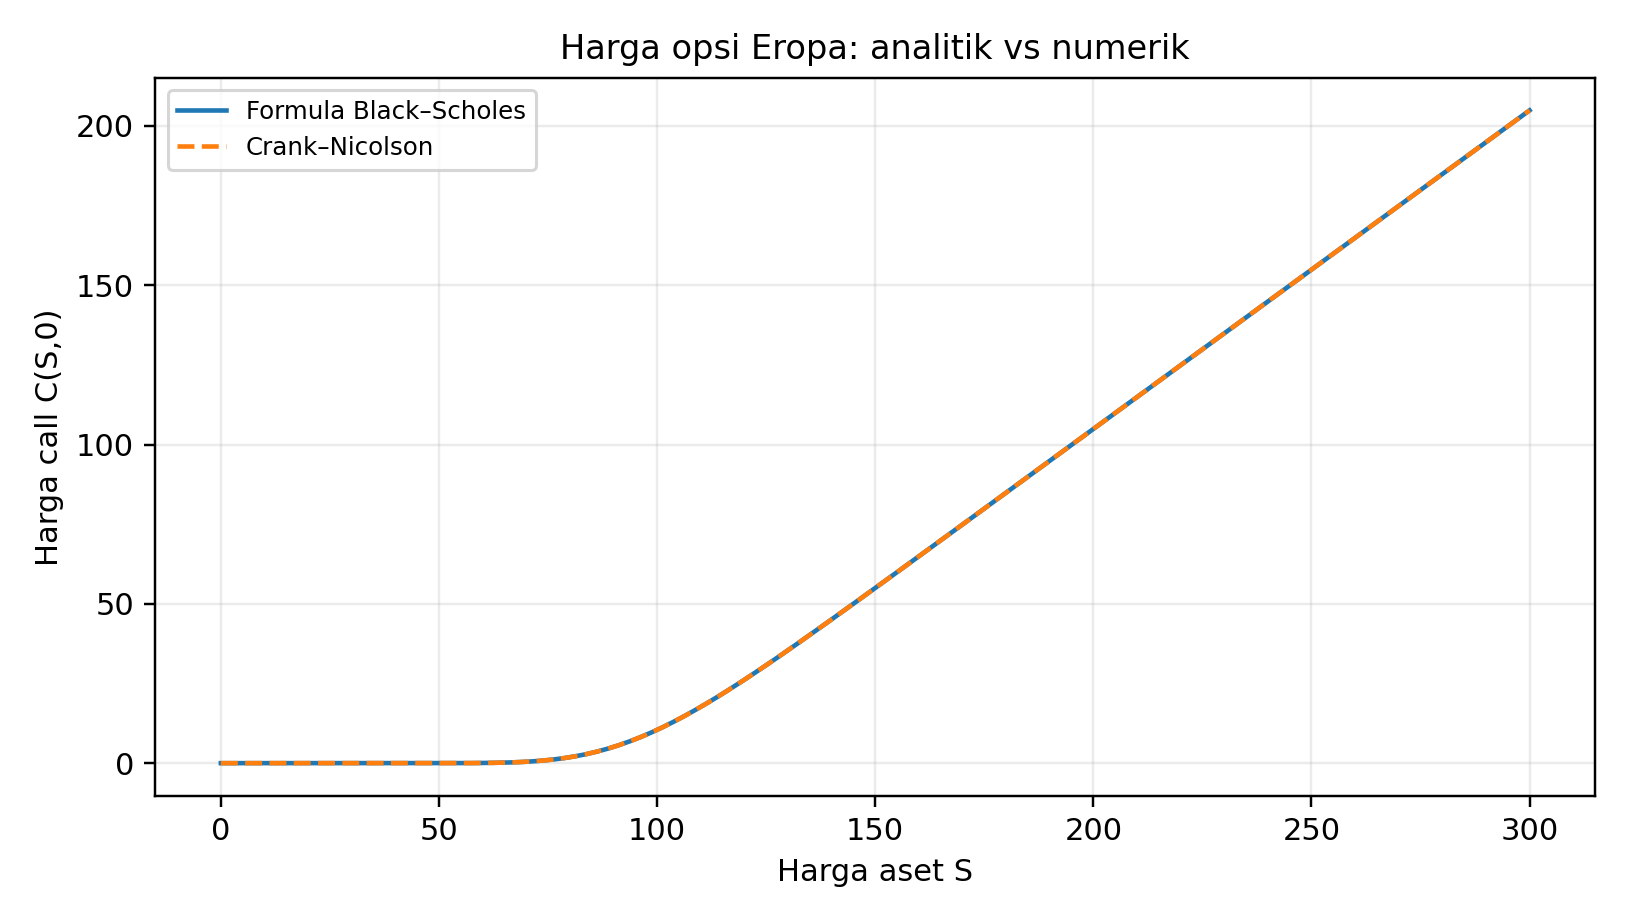
\includegraphics[width=\linewidth,height=4.7cm,keepaspectratio]{figures/black_scholes_compare.png}
\end{columns}
\end{frame}

% 19 ----------------------------------------------------------------
\begin{frame}{Galat Black--Scholes dan Peran Regularitas Data}
\begin{columns}[T,onlytextwidth]
\column{0.52\textwidth}
\centering
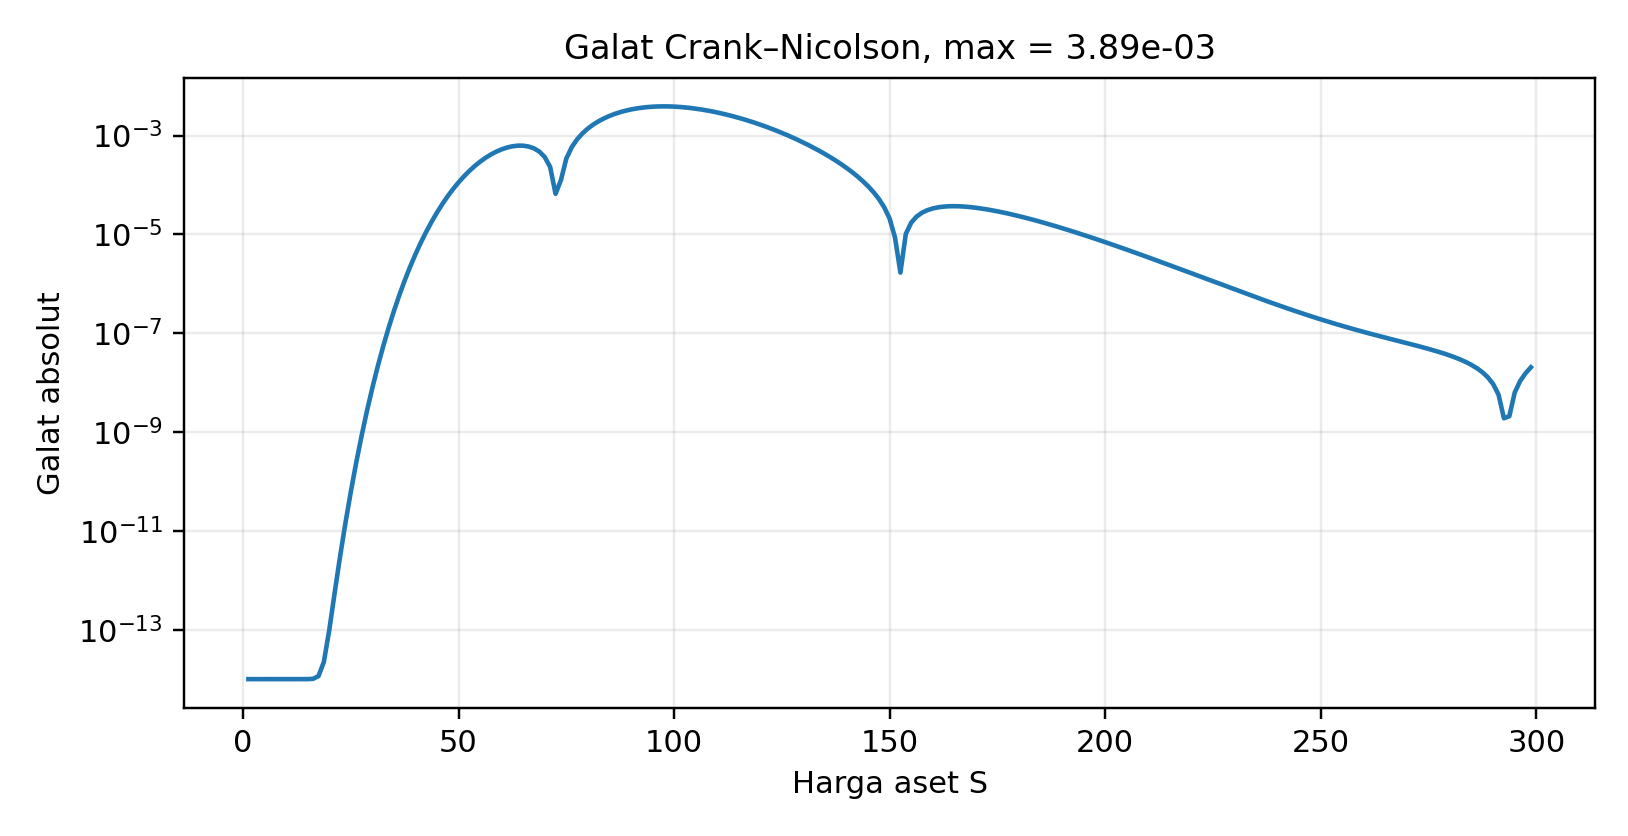
\includegraphics[width=\linewidth,height=3.8cm,keepaspectratio]{figures/black_scholes_error.png}
\column{0.45\textwidth}
\footnotesize
\begin{block}{Mengapa error besar dekat $S=K$?}
Payoff $\max(S-K,0)$ kontinu tetapi tidak terdiferensialkan di $S=K$. Data awal dalam variabel waktu-mundur tidak mulus di titik itu.
\end{block}
\begin{block}{Pelajaran numerik}
Skema yang stabil tetap perlu diperiksa terhadap solusi analitik, terutama dekat titik yang tidak mulus. Grid refinement dan start-up damping dapat diperlukan agar perilaku praktis sesuai orde teoritis.
\end{block}
\end{columns}
\pdpsource{Rannacher (1984), Numerische Mathematik 43, 309--327; Wade et al. (2007), J. Comput. Appl. Math. 204, 144--158.}
\end{frame}

% 20 ----------------------------------------------------------------
\begin{frame}{Difusi Tekanan pada Media Berpori: dari Konservasi ke Diffusion Equation}
\footnotesize
Ambil $p(\mathbf x,t)$ sebagai tekanan fluida. Untuk aliran Darcy, fluks volumetrik
\[
\boxed{\mathbf q=-\frac{\mathcal K}{\mu}\nabla p},
\]
dengan $\mathcal K$ permeabilitas dan $\mu$ viskositas. Untuk fluida/batuan sedikit kompresibel, neraca massa linear dapat ditulis
\[
\boxed{\phi c_t\,p_t+\nabla\cdot\mathbf q=s},
\]
dengan $\phi$ porositas, $c_t$ kompresibilitas total, dan $s$ sumber volumetrik.
Substitusi hukum Darcy memberi
\[
\phi c_t p_t=\nabla\cdot\left(\frac{\mathcal K}{\mu}\nabla p\right)+s.
\]
Jika $\mathcal K,\mu,\phi,c_t$ konstan, aliran 1D, dan $s=0$:
\[
\boxed{p_t=D p_{xx}},\qquad
\boxed{D=\frac{\mathcal K}{\phi\mu c_t}}.
\]
Model reservoir yang lebih kompleks dengan heterogenitas, geometri radial, atau sifat bergantung tekanan kembali pada bentuk umum sebelum penyederhanaan ini.
\end{frame}

% 21 ----------------------------------------------------------------
\begin{frame}{Benchmark Analitik Difusi pada Domain Semi-Takhingga}
\small
Normalisasi perubahan tekanan menjadi $u(x,t)$ dan ambil
\[
 u_t=D u_{xx},\qquad x>0,\ t>0,
\]
\[
 u(x,0)=0,\qquad u(0,t)=1,\qquad u(x,t)\to0\ \text{ketika }x\to\infty.
\]
Solusi similarity adalah
\[
\boxed{u(x,t)=\operatorname{erfc}\!\left(\frac{x}{2\sqrt{Dt}}\right)},
\]
dengan
\[
\operatorname{erfc}(z)=\frac{2}{\sqrt\pi}\int_z^\infty e^{-\xi^2}\,d\xi.
\]
\begin{columns}[T,onlytextwidth]
\column{0.58\textwidth}
\centering
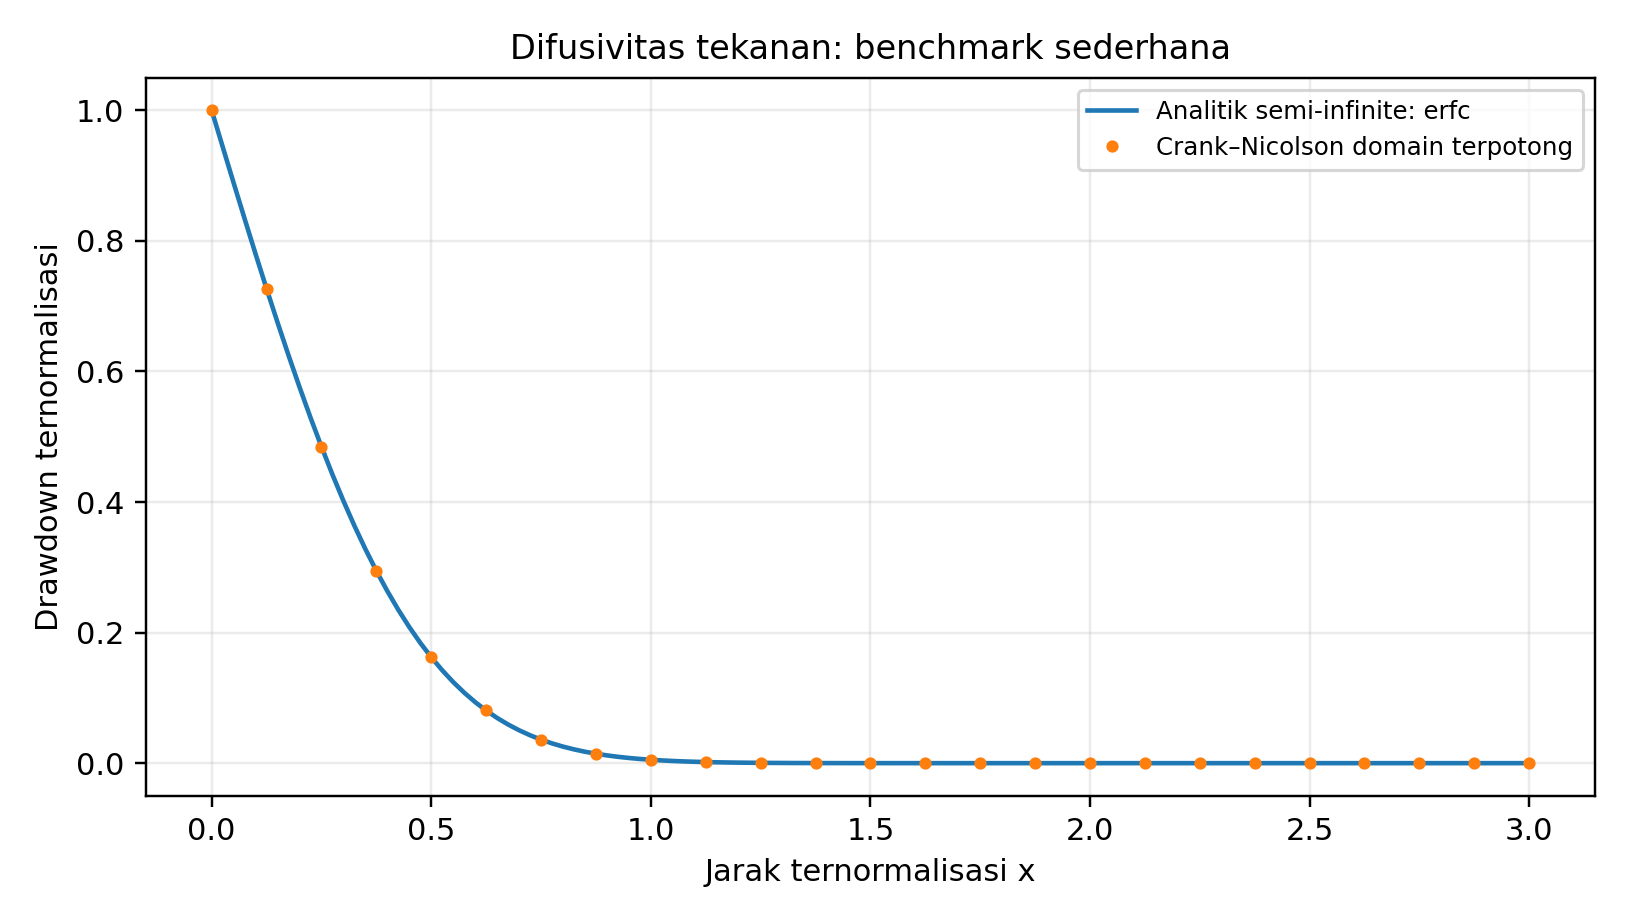
\includegraphics[width=\linewidth,height=2.9cm,keepaspectratio]{figures/reservoir_diffusion.png}
\column{0.38\textwidth}
\begin{block}{Verifikasi}
Pada komputer domain harus dipotong menjadi $0\le x\le L$. Karena itu error dapat berasal dari grid \emph{dan} dari pemilihan $L$ yang terlalu pendek.
\end{block}
\end{columns}
\end{frame}

% 22 ----------------------------------------------------------------
\begin{frame}{Dari Persamaan Panas ke Masalah Eliptik Tunak}
\small
Model konduksi panas dengan sumber volumetrik $Q$ adalah
\[
\boxed{\rho c_p T_t=\nabla\cdot(k_T\nabla T)+Q},
\]
dengan $\rho$ rapat massa, $c_p$ kalor jenis, dan $k_T$ konduktivitas termal.
Pada keadaan tunak,
\[
T_t=0,
\]
sehingga
\[
-\nabla\cdot(k_T\nabla T)=Q.
\]
Jika $k_T$ konstan,
\[
\boxed{-\Delta T=f},\qquad
\boxed{f=\frac{Q}{k_T}},
\]
dengan operator Laplace dua dimensi
\[
\boxed{\Delta T=T_{xx}+T_{yy}}.
\]
Jadi persamaan Poisson muncul sebagai limit keadaan tunak dari model difusi/konduksi dengan sumber.
\end{frame}

% 23 ----------------------------------------------------------------
\begin{frame}{Benchmark Analitik untuk Masalah Laplace pada Persegi Panjang}
\footnotesize
Sebelum Poisson dengan sumber umum, pertimbangkan Laplace
\[
 u_{xx}+u_{yy}=0,\qquad 0<x<L,\ 0<y<H,
\]
dengan
\[
 u(0,y)=u(L,y)=u(x,0)=0,
\qquad
 u(x,H)=\sin\left(\frac{\pi x}{L}\right).
\]
Ambil $u=X(x)Y(y)$. Separasi memberi
\[
\frac{X''}{X}=-\frac{Y''}{Y}=-\lambda.
\]
Syarat $X(0)=X(L)=0$ memilih mode pertama
\[
X(x)=\sin\left(\frac{\pi x}{L}\right),
\]
sedangkan
\[
Y''-\left(\frac{\pi}{L}\right)^2Y=0,
\qquad Y(0)=0.
\]
Setelah memenuhi $u(x,H)$,
\[
\boxed{u(x,y)=\sin\left(\frac{\pi x}{L}\right)
\frac{\sinh(\pi y/L)}{\sinh(\pi H/L)}}.
\]
Ini contoh lain bahwa basis Fourier/eigen yang telah dipelajari menyediakan benchmark eksak untuk solver eliptik.
\end{frame}

% 24 ----------------------------------------------------------------
\begin{frame}{Skema Lima Titik untuk Persamaan Poisson}
\footnotesize
Untuk grid seragam $x_i=ih$, $y_j=jh$, gunakan aproksimasi turunan kedua yang sama seperti pada persamaan panas:
\[
u_{xx}(x_i,y_j)=\frac{U_{i+1,j}-2U_{i,j}+U_{i-1,j}}{h^2}+O(h^2),
\]
\[
u_{yy}(x_i,y_j)=\frac{U_{i,j+1}-2U_{i,j}+U_{i,j-1}}{h^2}+O(h^2).
\]
Untuk $-\Delta u=f$ diperoleh
\[
\boxed{
\frac{4U_{i,j}-U_{i+1,j}-U_{i-1,j}-U_{i,j+1}-U_{i,j-1}}{h^2}=f_{i,j}}
\]
dengan galat pemotongan $O(h^2)$ untuk solusi yang cukup halus.
\begin{block}{Perbedaan dengan persamaan panas}
Tidak ada langkah waktu. Semua nilai interior harus dicari secara serempak dari sistem linear sparse
\[
\boxed{A\mathbf U=\mathbf b}.
\]
\end{block}
\end{frame}

% 25 ----------------------------------------------------------------
\begin{frame}{Manufactured Solution dan Uji Konvergensi Poisson}
\begin{columns}[T,onlytextwidth]
\column{0.49\textwidth}
\footnotesize
Pilih solusi yang sengaja diketahui
\[
 u(x,y)=\sin(\pi x)\sin(\pi y),
\]
yang memenuhi $u=0$ pada batas persegi satuan. Karena
\[
-\Delta u=2\pi^2\sin(\pi x)\sin(\pi y),
\]
maka ambil
\[
 f(x,y)=2\pi^2\sin(\pi x)\sin(\pi y).
\]
Setelah solver dijalankan, ukur galat maksimum
\[
E_h=\max_{i,j}|U_{i,j}-u(x_i,y_j)|.
\]
Untuk skema orde dua, $E_h\approx Ch^2$, sehingga orde teramati
\[
\boxed{p\approx\frac{\log(E_h/E_{h/2})}{\log 2}}\to 2
\]
ketika grid cukup halus.
\column{0.49\textwidth}
\centering
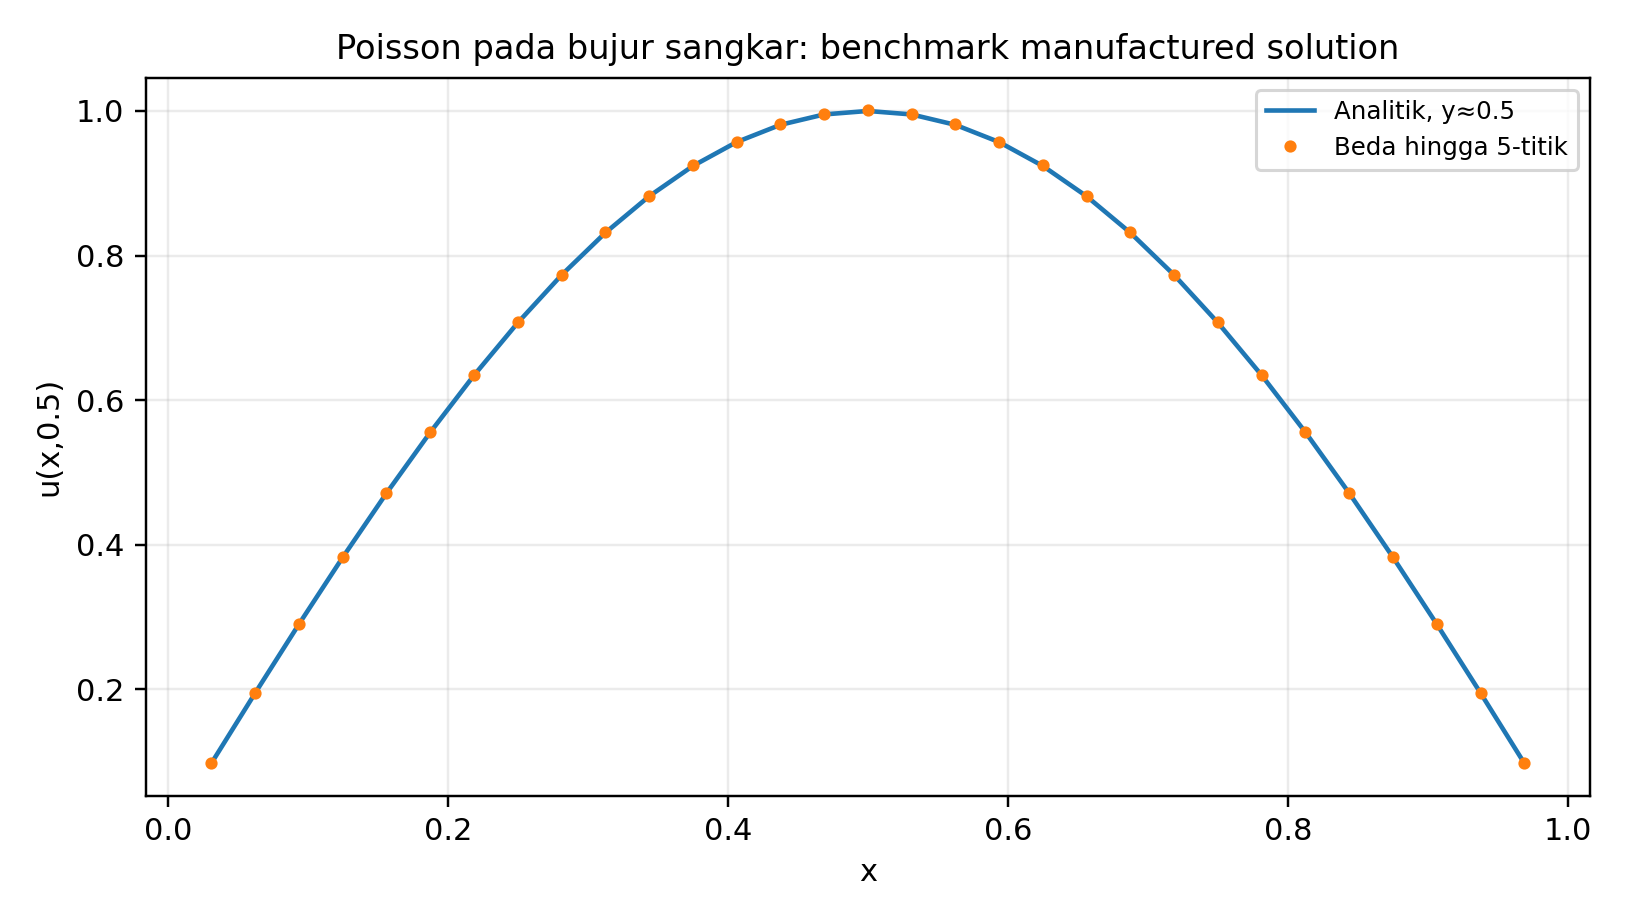
\includegraphics[width=\linewidth,height=2.9cm,keepaspectratio]{figures/poisson_compare.png}
\vspace{0.08cm}
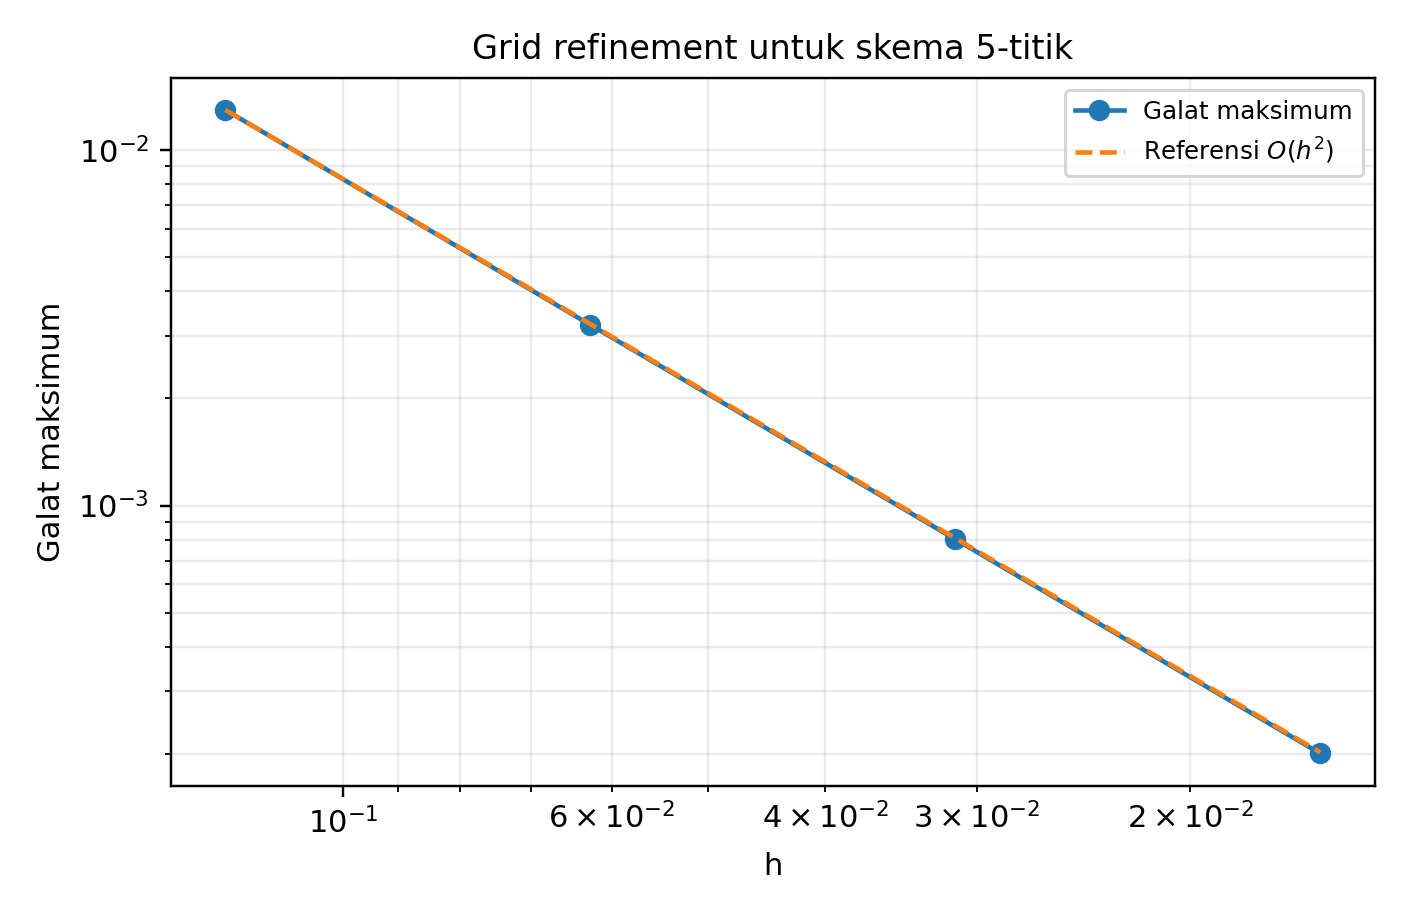
\includegraphics[width=\linewidth,height=1.9cm,keepaspectratio]{figures/poisson_convergence.png}
\end{columns}
\end{frame}

% 26 ----------------------------------------------------------------
\begin{frame}{Prosedur Pemilihan dan Verifikasi Metode Numerik PDP}
\small
\begin{enumerate}
\item \textbf{Formulasi model.} Nyatakan variabel, domain, asumsi, parameter, IC/BC, dan makna setiap suku.
\item \textbf{Cari kasus pembanding.} Sederhanakan model ke kasus yang masih mewakili mekanisme utama dan mempunyai solusi analitik; jika tidak tersedia, gunakan manufactured solution.
\item \textbf{Turunkan diskretisasi.} Setiap aproksimasi turunan harus berasal dari Taylor/integrasi/variational form yang jelas.
\item \textbf{Periksa konsistensi.} Tentukan galat pemotongan dan orde formal.
\item \textbf{Periksa stabilitas.} Gunakan analisis yang sesuai: mode Fourier/eigen, energy estimate, maximum principle, atau sifat matriks.
\item \textbf{Lakukan verifikasi.} Bandingkan dengan solusi eksak dan lakukan refinement.
\item \textbf{Kembalikan kompleksitas.} Terapkan solver pada model utama setelah perilaku pada benchmark dipahami.
\item \textbf{Validasi bila diperlukan.} Jika tujuan akhir adalah prediksi dunia nyata, bandingkan model dengan data relevan.
\end{enumerate}
\end{frame}

% 27 ----------------------------------------------------------------
\begin{frame}{Keterkaitan dengan Case 2}
\small
Struktur minimal analisis komputasi setiap kelompok:
\begin{columns}[T,onlytextwidth]
\column{0.31\textwidth}
\begin{block}{Model utama}
Fenomena nyata, asumsi, governing PDE, makna tiap suku, parameter, IC/BC, klasifikasi.
\end{block}
\column{0.31\textwidth}
\begin{block}{Benchmark analitik}
Kasus sederhana, solusi analitik/Fourier/eigen, atau manufactured solution yang dapat diperiksa.
\end{block}
\column{0.31\textwidth}
\begin{block}{Numerik dan interpretasi}
Diskretisasi, stabilitas, error, refinement, simulasi kasus utama, interpretasi dan validation bila data tersedia.
\end{block}
\end{columns}
\vspace{0.15cm}
\begin{beamercolorbox}[sep=.12cm,wd=\textwidth]{normal text}
\centering
Pola yang sama sudah terlihat pada shallow-water: sistem nonlinear yang kompleks memiliki limit amplitudo kecil yang menjadi persamaan gelombang dan mempunyai solusi analitik. Prinsip tersebut sekarang diterapkan pada difusi dan masalah eliptik.
\end{beamercolorbox}
\end{frame}

% 28 ----------------------------------------------------------------
\begin{frame}{Referensi Utama}
\scriptsize
\begin{thebibliography}{9}
\bibitem{dmn1} D. Michiko M. Noor (2026). \emph{Deret Fourier (I)--(III)}, materi Persamaan Diferensial Parsial, ITERA.
\bibitem{dmn2} D. Michiko M. Noor (2026). \emph{Persamaan Panas: Separasi Variabel}, materi Persamaan Diferensial Parsial, ITERA.
\bibitem{lax1956} Lax, P.D. \& Richtmyer, R.D. (1956). Survey of the stability of linear finite difference equations. \emph{Communications on Pure and Applied Mathematics}, 9, 267--293. DOI: 10.1002/cpa.3160090206.
\bibitem{cn1947} Crank, J. \& Nicolson, P. (1947). A practical method for numerical evaluation of solutions of partial differential equations of the heat-conduction type. \emph{Proc. Cambridge Philosophical Society}, 43, 50--67. DOI: 10.1017/S0305004100023197.
\bibitem{bs1973} Black, F. \& Scholes, M. (1973). The Pricing of Options and Corporate Liabilities. \emph{Journal of Political Economy}, 81(3), 637--654. DOI: 10.1086/260062.
\bibitem{rannacher1984} Rannacher, R. (1984). Finite element solution of diffusion problems with irregular data. \emph{Numerische Mathematik}, 43, 309--327. DOI: 10.1007/BF01390130.
\bibitem{roache2002} Roache, P.J. (2002). Code Verification by the Method of Manufactured Solutions. \emph{Journal of Fluids Engineering}, 124(1), 4--10. DOI: 10.1115/1.1436090.
\end{thebibliography}
\vspace{0.04cm}
\pdpnote{Textbook pendamping: Strikwerda, \emph{Finite Difference Schemes and Partial Differential Equations}; Morton \& Mayers, \emph{Numerical Solution of Partial Differential Equations}; LeVeque, \emph{Finite Difference Methods for Ordinary and Partial Differential Equations}.}
\end{frame}

\end{document}
